%
%  DBS-Project
%
%  NvG, FH, SR
%
\documentclass[11pt,german]{scrartcl}

% See geometry.pdf to learn the layout options.
\usepackage{geometry}
\geometry{a4paper}

% To begin paragraphs with an empty line
\usepackage[parfill]{parskip}

% Use utf-8 encoding for foreign characters
\usepackage[utf8]{inputenc}
\usepackage[T1]{fontenc}

% Setup for fullpage use
\usepackage{fullpage}

% More symbols
\usepackage{amsmath}
\usepackage{amssymb}
%\usepackage{latexsym}

% Package for including code in the document
\usepackage{listings}
\usepackage{color}
\usepackage{moreverb}

% This is now the recommended way for checking for PDFLaTeX:
\usepackage{ifpdf}

%\newif\ifpdf
%\ifx\pdfoutput\undefined
%\pdffalse % we are not running PDFLaTeX
%\else
%\pdfoutput=1 % we are running PDFLaTeX
%\pdftrue
%\fi

\ifpdf
\usepackage[pdftex]{graphicx}
\else
\usepackage{graphicx}
\fi


\title{Objektmodell: Design}
\author{Felix Höffken, Sebastian Raitza, Nico von Geyso}

% Activate to display a given date or no date
\date{}

%%%%%%%%%%%%%%%%%%%%%%%%%%%%%%%%%%%%%%%%%%%%%%%%%%%%%%%%%%%%%%%%%%
\begin{document}

\renewcommand{\labelenumi}{\alph{enumi})}
\renewcommand{\labelenumii}{$\bullet$}

% define a macro ausgabe which takes as argument
% your ausgabe.txt file’s name 
% \newcommand{\ausgabe}[1] {\hrule\small\verbatiminput{#1}\normalsize\hrule}

\definecolor{light-gray}{gray}{0.95}

\lstset{
  language=Java,               % choose the language of the code
  basicstyle=\scriptsize,   % size of fonts used for the code
  numbers=left,             % where to put the line-numbers
  numberstyle=\tiny,        % size of fonts for used line-numbers
  stepnumber=1,             % step between line-numbers
  numbersep=5pt,            % how far the line-numbers are from the code
  backgroundcolor=\color{light-gray},  % background color, add \usepackage{color}
  showspaces=false,         % show spaces adding particular underscores
  showstringspaces=false,   % underline spaces within strings
  showtabs=false,           % show tabs within strings adding particular underscores
  frame=single,             % adds a frame around the code
  tabsize=4,                % sets default tabsize to 2 spaces
  captionpos=b,             % sets the caption-position to bottom
  breaklines=true,          % sets automatic line breaking
  breakatwhitespace=false,  % sets if automatic breaks should only happen at whitespace
  escapeinside={\%*}{*)},   % if you want to add a comment within your code
  extendedchars=true,
  literate=%
    {Ö}{{\"O}}1
    {Ä}{{\"A}}1
    {Ü}{{\"U}}1
    {ß}{{\ss}}2
    {ü}{{\"u}}1
    {ä}{{\"a}}1
    {ö}{{\"o}}1
    {°}{{}}0
}


\maketitle

%%%%%%%%%%%%%%%%%%%%%%%%%%%%%%%%%%%%%%%%%%%%%%%%%%%%%%%%%%%%%%%%%%

%\setcounter{section}{5}

%\clearpage
\section{Klassendiagramm}
Alle Klassen sind auch als Diagramm in den Dateien {\it objektdiagramm\_entity.pdf} und {\it objektdiagramm\_permission.pdf} zu finden.

\section{Packet: dbs.project.entity}

\begin{description}

\item [Advisor]
Ein Advisor repräsentiert einen Betreuer, also eine Person, die für ein Team arbeitet (z.B. Trainer, Teamarzt, ...).

\item [Country]
Country repräsentiert ein Land.

\item [GroupMatch]
Ein GroupMatch ist ein Spiel, dass in der Gruppenphase ausgetragen wird.

\item [GroupStage]
Die GroupStage ist die Gruppenphase des Turniers.

\item [KnockOutMatch]
Ein KnockOutMatch ist ein Spiel, dass in der KO-Runde ausgetragen wird.

\item [Match]
Ein Match ist ein Spiel, also die Oberklasse von KnockOutMatch und GroupMatch. Sie ist {\it abstact} kann also nicht implementiert werden.

\item [MatchEvent]
Ein MatchEvent ist ein Event, dass während eines Spiels auftreten kann. Es ist {\it abstact} kann also nicht direkt implementiert werden.
Es gibt mehrere Unterklassen, die später erklärt werden.

\item [Person]
Eine Person ist eine Person, die in dem Turnier auftritt. Sie ist {\it abstract} und die Überklasse von Player und Advisor.

\item [Player]
Ein Player repräsentiert einen Spieler im Turnier.

\item [Stadium]
Ein Stadium repräsentiert ein Stadion.

\item [Team]
Ein Team ist eine Gruppe aus Advisorn und Spielern, usw. Sie repräsentieren die Mannschafte, die gegeneinander spielen.

\item [Tournament]
Ein Tournament ist ein Turnier - da mehrere Turniere in unsere Datenbank passen sollen ist sie nötig.

\item [TournamentGroup]
Eine TournamentGroup repräsentiert eine Gruppe in der Gruppenphase (Gruppe A, B, C, ...) .

\end{description}

\section{Packet: dbs.project.entity.event}
Diese Entitäten implementieren die abstrakte Klasse MatchEvent.

\begin{description}

\item [MatchEndEvent]
Ein MatchEndEvent repräsentiert den Schlusspfiff in einem Spiel.

\item [PlayerEvent]
Ein PlayerEvent ist ein im Spiel auftretendes Ereignis, das einen Spieler betrifft. Die Klasse ist {\it abstract} und wird von CardEvent, GoalEvent, LineUpEvent und SubstitutionEvent implementiert.

\end{description}

\begin{figure}[htb]
\begin{center}
\leavevmode
\includegraphics[height=0.75\textheight,angle=90]{../diagrams/objektdiagramm_entity.pdf}
\end{center}
\caption{Objektmodell: WM}
\label{fig:entities}
\end{figure}



\section{Packet: dbs.project.entity.event.player}
Diese Klassen implementieren die abstrakte Klasse PlayerEvent.

\begin{description}
\item [CardEvent]
Ein CardEvent repräsentiert die Vergabe einer Karte an einen Spieler.

\item [GoalEvent]
Ein GoalEvent repräsentiert ein (Eigen-)Tor.

\item [LineUpEvent]
Ein LineUpEvent repräsentiert das Aufstellen eines Spielers in der Startelf.

\item [SubstitutionEvent]
Ein SubstitutionEvent repräsentiert das Auswechseln bzw. Einwechseln eines Spielers.
\end{description}

\section{Packet: dbs.project.entity.permission}
Diese Entitäten werden zur Authentifizierung und Rechtevergabe benötigt.

\begin{description}
\item [Actor]
Ein Actor repräsentiert einen Akteur, der Daten in die Datenbank speichern, oder Daten aus ihr lesen will.

\item [Permission]
Permissions verwalten den Zugang zu gewissen Ressourcen im System.

\item [Resource]
Eine Ressource spiegelt ein Recht auf eine Entität wieder. Hat ein Akteur also die Berechtigung (Permission) für eine Ressource, so kann er diese je nach vergebener Berechtigung einsehen oder verwalten.

\item [Role]
Akteuren können gewisse Rollen zugewiesen werden. Diese haben wieder je nach Einstellung Berechtigungen auf Ressourcen.
\end{description}

\begin{figure}[htb]
\begin{center}
\leavevmode
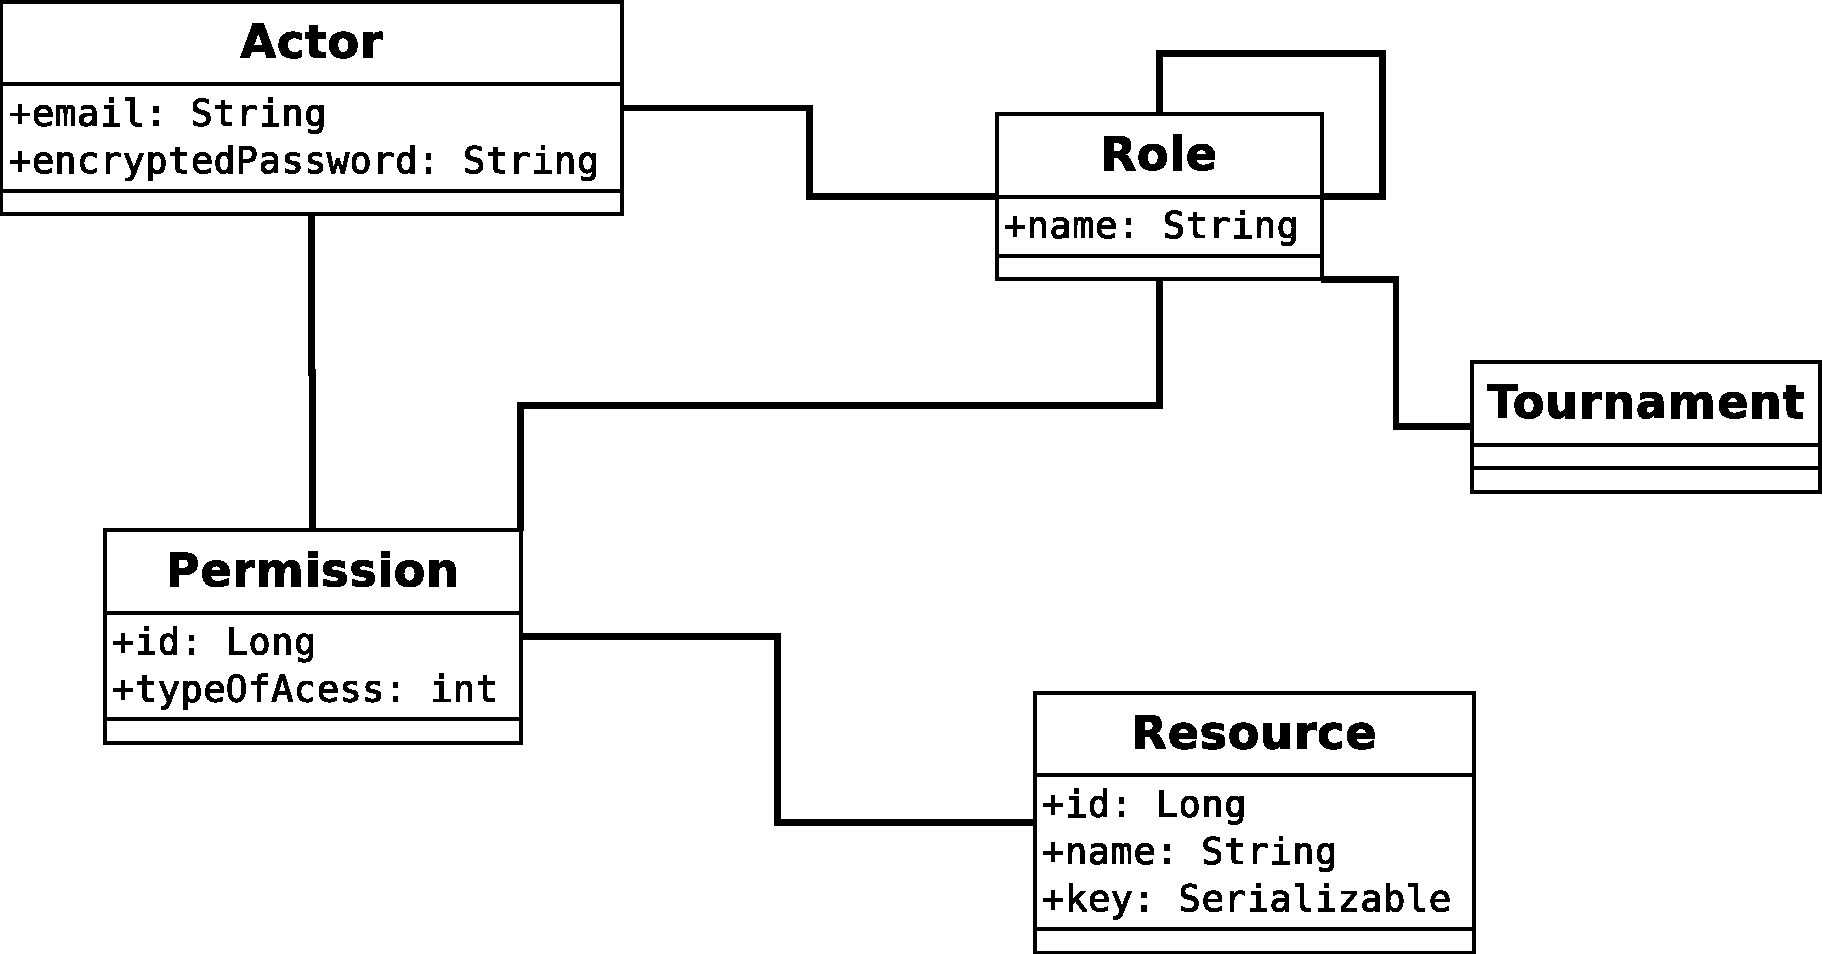
\includegraphics[width=\textwidth]{../diagrams/objektdiagramm_permission.pdf}
\end{center}
\caption{Objektmodell: Authentifizierung und Rechtevergabe}
\label{fig:permission}
\end{figure}

\end{document}
